\section{Full detection in two-hop routing}
\label{sec:full_detect}

\begin{figure}
  \centering
  {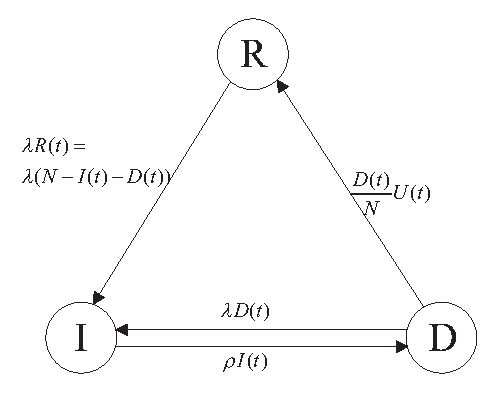
\includegraphics[width=0.25\textwidth]
  {fig/state_transition_detect.eps}}
     \caption{State transition of the relay nodes.}
     \label{fig:ss_dt}
\end{figure}
%\subsection{Analysis of prob=$\frac{M}{I+M}$}
%\begin{small}
%\begin{equation}\label{eq:IandM_wod}
%%\nonumber
%\begin{aligned}
%\dot{I} &= \beta (N-I) - \rho I,\\
%\dot{M} &= \rho I - \beta M - \frac{M}{I+M} U_{m},\\
%\dot{H} &= - \beta (N-I-M) + \frac{M}{I+M} U_{m},
%\end{aligned}
%\end{equation}
%\end{small}
%when $0 \le I(t) \le N$ and $0 \le M(t) \le N$.
%At first, $M(0)=0$ and $I(0)=0$.
%Thus
%\begin{small}
%\begin{equation}\label{eq:It_wod}
%%\nonumber
%\begin{aligned}
%I(t) = \frac{ \beta N }{ \beta + \rho } - \frac{ \beta N }{ \beta + \rho } e^{-(\beta + \rho)t},
%\end{aligned}
%\end{equation}
%\end{small}
%still holds.
%Here
%\begin{small}
%\begin{equation}\label{eq:It_wod}
%%\nonumber
%\begin{aligned}
%I \dot{M} + M \dot{M} = -\beta M^2 + (\rho I - \beta I - U_{m}) M + \rho I^2.
%\end{aligned}
%\end{equation}
%\end{small}
%$M(t)$ is solved by the Runge-Kutta method.*
%
%\subsection{Analysis of prob=$\frac{M}{N}$}
%However,
The detection rate is $U_{m}$.
For each detection, a node will be chosen randomly from $N$ nodes.
Thus the probability that find the blackhole node is $\frac{M}{N}$.
\begin{small}
\begin{equation}
\nonumber
\begin{aligned}
\dot{I} &= \beta (N-I) - \rho I,\\
\dot{M} &= \rho I - \beta M - \frac{M}{N} U_{m},\\
\dot{S} &= - \beta (N-I-M) + \frac{M}{N} U_{m},
\end{aligned}
\end{equation}
\end{small}
So
\begin{small}
\begin{equation}
\nonumber
\begin{aligned}
I(t) = \frac{ \beta N }{ \beta + \rho } - \frac{ \beta N }{ \beta + \rho } e^{-(\beta + \rho)t},
\end{aligned}
\end{equation}
\end{small}
Then
\begin{small}
\begin{equation}
\nonumber
\begin{aligned}
\dot{M} + (\beta + \frac{U_{m}}{N})M = \rho I
\end{aligned}
\end{equation}
\end{small}

\begin{small}
\begin{equation}
\nonumber
\begin{aligned}
& M(t) \\
=& C e^{\int -(\beta + \frac{U_{m}}{N}) dt} + e^{\int -(\beta + \frac{U_{m}}{N}) dt} \int \rho I e^{\int (\beta + \frac{U_{m}}{N}) dt} dt \\
=& C e^{-(\beta + \frac{U_{m}}{N})t} + e^{-(\beta + \frac{U_{m}}{N})t} \rho \frac{ \beta N }{ \beta + \rho }  \int ( 1 - e^{-(\beta + \rho)t} ) e^{(\beta + \frac{U_{m}}{N})t} dt \\
=& C e^{-(\beta + \frac{U_{m}}{N})t} + \frac{ \rho \beta N }{ \beta + \rho } \frac{1}{\beta + \frac{U_{m}}{N}}
- \frac{ \rho \beta N }{ \beta + \rho } \frac{1}{\frac{U_{m}}{N} - \rho} e^{-(\beta + \rho)t}
\end{aligned}
\end{equation}
\end{small}
Because of $M(0) = 0$.
\begin{small}
\begin{equation}
\nonumber
\begin{aligned}
M(t) =& \frac{ \rho \beta N }{ \beta + \rho } \frac{1}{\beta + \frac{U_{m}}{N}}
- \frac{\rho \beta N}{(\beta + \frac{U_{m}}{N})(\frac{U_{m}}{N} - \rho)}  e^{-(\beta + \frac{U_{m}}{N})t}\\
& - \frac{ \rho \beta N }{ \beta + \rho } \frac{1}{\frac{U_{m}}{N} - \rho} e^{-(\beta + \rho)t}
\end{aligned}
\end{equation}
\end{small}

Here we find that ()\% reward is wasted in the selfish node.
Although the wasted reward is reduced because of the detection,
the additional cost,
which is caused by the detection behavior,
i.e., energy, bandwidth and wireless communication charge.
is introduced.
